\chapter{Un tour de C}
\label{cha:tour}
\thispagestyle{empty}

%% Calculate how old C is...
\newcount\cdifference\cdifference=\the\year\advance\cdifference by -1970

C is al een oude taal. De taal is rond 1970 ontworpen door Dennis Ritchie\footnote{Dennis MacAlister Ritchie (1941 -- 2011). Hij was de ontwerper van de programmeertaal C en was een van de ontwerpers van Unix. Bekende afgeleiden van Unix zijn Linux en FreeBSD.} en is dus al zo'n \the\cdifference\ jaar oud. Hij was bezig met het schrijven van een besturingssysteem (Engels: operating system)\footnote{Een besturingssysteem is een programma dat draait op een computer en zorgt voor het beschikbaar stellen van \textsl{resources} aan de gebruiker (lees: programma's). Zo zorgt een besturingssysteem ervoor dat de bestanden op de harde schijf netjes worden opgeslagen en beschikbaar zijn. Daarnaast zorgt een besturingssysteem ervoor dat programma's netjes naast elkaar kunnen draaien. Drie bekende besturingssystemen zijn Windows, Linux en OS-X.} en zocht naar een mogelijkheid om dit te schrijven op een hoger niveau dat gebruikelijk voor die tijd. In die tijd werden besturingssystemen geschreven in assembly, een taal die dicht de hardware van de computer ligt. Programma's schrijven in assembly is tijdrovend en gevoelig voor fouten van de programmeur.

C is een zogenoemde derde-generatie-taal (3GL) en zorgt ervoor dat programma's gestructureerd kunnen worden geschreven zonder dat de programmeur kennis hoeft te hebben van de hardware waarop het programma draait. Toch biedt de taal constructies om die hardware in te stellen, een voorwaarde voor het schrijven van een operating system. Daarom is de taal geliefd bij programmeurs van kleine computersystemen waarop geen operating system draait, de zogenoemde \textsl{bare metal systems}. Het is vaak ook de enige taal die gebruikt kan worden op dit soort systemen, naast assembly.

C is geschreven voor ervaren programmeurs die behoefte hebben voor het schrijven van compacte programma's, dat te zien is in de vele, soms onduidelijke, taalconstructies. Het is eigenlijk niet geschikt voor beginnende programmeurs. Het is zeker mogelijk om programma's te schrijven die niet correct werken, maar met enige discipline kan ook de minder ervaren programmeur de taal prima gebruiken.

C is een algemeen bruikbare taal (\textsl{general purpose language}) en is dus niet voor een specifiek doeleind ontworpen (behalve voor het schrijven van operating systems). Zo kunnen met C wiskundige berekeningen worden uitgevoerd maar de programmeur moet zelf alles schrijven. Er zijn wel \textsl{functies} beschikbaar voor bijvoorbeeld sinus, cosinus en tangens. Er zijn echter talen die dit veel beter ondersteunen. Ook het verwerken van bestanden is mogelijk maar het manipuleren van \textsl{strings} (een rij karakters) moet door de programmeur zelf worden uitgewerkt. Ook hier zijn diverse functies beschikbaar die het programmeerwerk enigszings verlichten.

C is een \textsl{imperatieve} programmeertaal, een van de bekende programmeerparadigma's\footnote{Een programmeerparadigma is een manier van programmeren en een wijze waarop een programma wordt vormgegeven.}.
C moet concurreren met vele andere talen zoals C++, C\#, Python en Java. C++ is ontwikkeld door Bjarne Stroustrup als ``de betere C'' en ondersteunt \textsl{objectgeoriënteerd} programmeren. C\# is ontwikkeld door MicroSoft en is de \textsl{de facto} programmeertaal op Windows-systemen. Python is ontwikkeld door het Centrum voor Wiskunde en Informatica van de Universiteit van Amsterdam. 

\section{De computer}
Een \textsl{computer}\index{computer} is een elektronisch, digitaal systeem dat \textsl{data} verwerkt aan de hand van een lijst \textsl{instructies}\index{instructie}. Het Engelse woord voor verwerken is ``to process''. En daar komt de naam vandaan van een belangrijk onderdeel van de computer: de \textsl{processor}\index{processor}. 

De instructies die de processor kan uitvoeren zijn zeer eenvoudig. Voorbeelden zijn ``tel op'' en ``trek af'' en ``bepaal of het ene getal kleiner is dan het andere getal''. Een processor kan niet in één keer ``doe dit tien keer en bereken de wortel van diverse getallen en druk af op het scherm'' uitvoeren. Als we dat willen, dan moeten we dit opdelen in de eenvoudige instructies die de processor wel kan verwerken. Alle instructies bij elkaar wordt een \textsl{programma}\index{programma} genoemd en de verzamelnaam voor alle programma's wordt \textsl{software}\index{software} genoemd.

Een computer heeft naast de processor \textsl{geheugen}\index{geheugen} om de data en instructies op te slaan. Er zijn twee soorten geheugens: ROM\index{ROM} (Read Only Memory) is een geheugen waarvan de inhoud niet gewijzigd kan worden; RAM\index{RAM} (Random Access Memory) is geheugen waarvan de inhoud wel gewijzigd kan worden. Over het algemeen wordt het programma in de ROM opgeslagen en wordt de data in de RAM opgeslagen.

Naast ROM en RAM heeft de computer nog invoer- en uitvoermogelijkheden, anders is er geen communicatie met de buitenwereld mogelijk. De verzamelnaam is \textsl{I/O}\index{I/O} dat ``input'' en ``output'' betekent. Het is best lastig om de invoer en uitvoer te realiseren. Daarom wordt bij de gangbare computers een stuk software geladen (of het is al aanwezig in de ROM) om dat voor de gebruiker (en programmeur) te vereenvoudigen. Die software wordt een \textsl{besturingssysteem}\index{besturingssyteem} genoemd, maar gangbaar is om de Engelse naam Operating System\index{operating system} te gebruiken. Bekende besturingssytemen zijn Windows, Mac OS-X en Linux.

Niet alle gegevens zijn in het geheugen van de computer aanwezig. Een computer heeft (vaak) \textsl{secundair geheugen}\index{secundair geheugen}. Voorbeelden van secundair geheugen zijn harddisk (harde schijf), USB-sticks en SD-cards. De informatie op deze geheugendragers blijft aanwezig ook al wordt de computer uitgezet en weer aangezet. Om de informatie beschikbaar te maken worden de gegevens in \textsl{bestanden}\index{bestand} (Engels: file) gezet. De manier waarop dat wordt gerealiseerd wordt een \textsl{bestandssysteem}\index{bestandssysteem} (Engels: file system) genoemd. Bekende bestandssystemen zijn NTFS op Windows en ext3 op Linux. Het besturingssysteem zorgt ervoor dat de bestanden op ordentelijke wijze kunnen worden benaderd.

In de praktijd komen twee soorten computers tegen: de algemeen bruikbare computers waarop een besturingssysteem draait (PC, laptops) en dat grote hoeveelheid aan verschillende programma's kan uitvoeren en de zogenoemde \textsl{embedded systems}\index{embedded system}. Een embedded system in meestal geschikt om één taak uit te voeren en is voorzien van een kleine processor met geheugen en I/O-faciliteiten. Al deze componenten zijn op één ic (Integrated Circuit of chip genoemd)\index{chip} geplaatst. We noemen zo'n processorsysteem een \textsl{microcontroller}\index{microcontroller}. Voorbeelden van embedded systems zijn (de besturingen van) wasmachines, koelkasten, televisies, thermostaten, horloges en bloeddrukmeters. De markt voor embedded systems is trouwens vele malen groter dan de markt voor algemene bruikbare computers.

De microcontroller heeft meestal geen besturingssysteem. Dat noemen we \textsl{bare metal}\index{bare metal} systemen. Dat betekent dat de programmeur alles zelf moet ontwikkelen. Gelukkig leveren fabrikanten ontwikkelsystemen om programma's voor microcontrollers te produceren. Dat worden \textsl{compiler suites} of \textsl{toolchains}\index{toolchain} genoemd.


\section{De compiler}
C is een zogenoemde derde-generatie-taal. De broncode van een C-programma is voor een mens gewoon te lezen. Deze broncode kan niet direct door de processor worden uitgevoerd. De \textsl{C-compiler}\index{compiler} vertaalt de broncode naar instructies die de processor wel kan uitvoeren. Dat vertalen wordt \textsl{compileren}\index{compileren} genoemd. De instructies worden in bitpatronen in het geheugen opgeslagen. De bitpatronen noemen we \textsl{machinecode}\index{machinecode}. Elk type processor heeft zijn eigen verzameling bitpatronen, dat wordt de \textsl{Instruction Set Architecture}\index{ISA} genoemd. De ISA van een Intel-processor is dus anders dan die van een ATmega-processor, maar we kunnen wel zeggen dat elke processor ongeveer dezelfde soort instructies bevat. De C-compiler moet weten voor welke processor een C-programma wordt vertaald.

De C-programma kan niet worden uitgevoerd door de computer. We moeten eerst een programma compileren zodat instructies worden gegenereerd die de processor wel kan uitvoeren. Het vertaalde programma wordt een \textsl{uitvoerbaar bestand}\index{uitvoerbaar bestand} of \textsl{executable}\index{executable} genoemd. Een uitvoerbaar bestand wordt net als een C-programma opgeslagen op de harddisk. Bij het ontwikkelen van programma's voor microcontrollers wordt gebruik gemaakt van PC of laptop met een besturingssysteem en een toolchain. We noemen zo'n compiler een \textsl{cross compiler}\index{cross compiler}. De uitvoerbare instructies worden via de PC in het geheugen van de microcontroller \textsl{geprogrammeed}\index{programmeren}.

In het licht van het compilatieproces noemen we nog twee begrippen die we vaak zullen gebruiken: \textsl{compile-time}\index{compile-time} en \textsl{runtime}\index{runtime}. Met compile-time bedoelen we dat iets tijdens compileren van een C-programma bekend moet zijn. Een voorbeeld hiervan is het bepalen van de grootte van een variabele. Met runtime bedoelen we dat tijdens het uitvoeren van een programma iets wordt bepaald, bijvoorbeeld hoe vaak iets moet worden uitgerekend.

Hoewel een derde-generatie-taal suggereert dat we een C-programma door verschillende compilers kunnen laten vertalen en op verschillende computersystemen (lees: processoren) kunnen uitvoeren, moeten we helaas opmerken dat dat niet het geval is. Het is zeker mogelijk om een programma te schrijven dat door de Microsoft C-compiler en door de GNU C-compiler kan worden vertaald. Maar er zijn ook veel verschillen. Zo kan de grootte van gegevens door verschillende compilers op verschillende wijze worden geïnterpreteerd. Ook het bestandssysteem is op computers verschillend. Windows en Linux doen dat op hun eigen wijze. Het is dus best lastig om een programma te schrijven dat op beide besturingssystemen zonder problemen draait. En wat te denken van een microcontroller dat niet eens een bestandssysteem heeft. Daar heeft het bewerken van bestanden geen zinnige betekenis.


\section{Bibliotheken en functies}
Stel dat we een klein stukje C-programma hebben geschreven dat iets voor ons uitrekent, bijvoorbeeld het gemiddelde van een aantal getallen. We willen dit stukje programma vaker gebruiken in een groot C-programma. Dan plaatsen we de berekening in een \textsl{functie}\index{functie}. We kunnen nu in ons C-programma de functie meerdere malen \textsl{aanroepen}. De functie hoeft dus maar één keer geprogrammeerd te worden om meerdere keren gebruikt te worden.

Er zijn ook functies die al geschreven zijn, zoals het afdrukken van tekst op het scherm. We hoeven dus niet zelf een functie te schrijven die dat voor ons doet. Als deze functies zijn ondergebracht in \textsl{bibliotheken}\index{bibliotheek} (Engels: library)\index{library}. Als tijdens het compileren zo'n functie nodig is, dan zoekt de compiler in de bibliotheek of de functie beschikbaar is. De compiler ``plakt'' dan de functie bij het programma. Dat plakken wordt \textsl{linken}\index{linken} genoemd.

Bij de C-compiler wordt een zeer uitgebreide bibliotheek geleverd, de zogenoemde \textsl{standard library}\index{standard library}. De standard library bevat functies voor het afdrukken van tekst en gegevens, het bewerken van bestanden en het manipuleren van \textsl{strings}\index{string} (een stukje tekst opgeslagen in het geheugen). Daarnaast wordt ook de \textsl{mathematical library} meegeleverd waarin functies voor het berekenen van sinus, cosinus, logaritmen en e-machten zijn opgeslagen. Tijdens het compileren moet opgegeven worden dat moet worden gezocht in de bibliotheken.


\section{Ontwikkelsystemen}
De meeste boeken gaan uit van een \textsl{command line interface} op een Unix-derivaat. Met behulp van een \textsl{editor} wordt een programma ingevoerd en wordt op de commandoregel de C-compiler gestart. Daarna wordt het programma (ook via de commandoregel) gestart.
Natuurlijk is het ook mogelijk om alles met behulp van de command line te doen. Deze werkwijze wordt veel gebruikt op Linux-systemen maar kan ook op Windows worden gebruikt. Een voorbeeld is te zien in onderstaande figuur.

\begin{dosbox}
C:\textbackslash Users\textbackslash C> notepad mooi.c \hfill\textrm{(start Notepad)} \\
C:\textbackslash Users\textbackslash C> gcc -o mooi.exe mooi.c \hfill\textrm{(start C-compiler)}\\
C:\textbackslash Users\textbackslash C> .\textbackslash mooi.exe \hfill\textrm{(start uitvoerbaar programma)}\\
C is een mooie taal \hfill\textrm{(de uitvoer op het scherm)}\\
C:\textbackslash Users\textbackslash C>
\end{dosbox}

Dit is echter niet de werkwijze van veel programmeurs. Gelukkig zijn er goede ontwikkelsystemen (IDE: Integrated Development Environment) die het programmeerwerk verlichten. Bekende systemen zijn Microsoft Visual Studio, Code::Blocks en Apple's Xcode.
Zulke ontwikkelsystemen zorgen ervoor dat de programmeur gemakkelijk het programma kan invoeren, de compiler kan starten en het programma kan \textsl{debuggen}\index{debuggen}. Dat laatste is vaak nodig omdat blijkt dat (de uitvoer) een programma niet verloopt zoals de programmeur voor ogen had. Met debuggen wordt het programma stap voor stap doorlopen en kan de programmeur (of is het debugger) de inhoud van \textsl{variabelen}\index{variabele} bekijken. Ook kan de programmeur bepalen of de \textsl{statements}\index{statement} (opdrachten voor de computer) op de juiste volgorde worden uitgevoerd.

Een voorbeeld van Microsoft Visual Studio is te zien in figuur~\ref{fig:unvs2019}. Visual Studio ondersteunt het ontwikkelen van software voor Windows-computers met behulp van een groot aantal talen: C, C++, C\#, Python. Het is zelfs mogelijk om software te ontwikkelen voor Linux-systemen. Een korte introductie wordt gegeven in bijlage~\ref{cha:visualstudio}.

\begin{figure}[!ht]
\centering
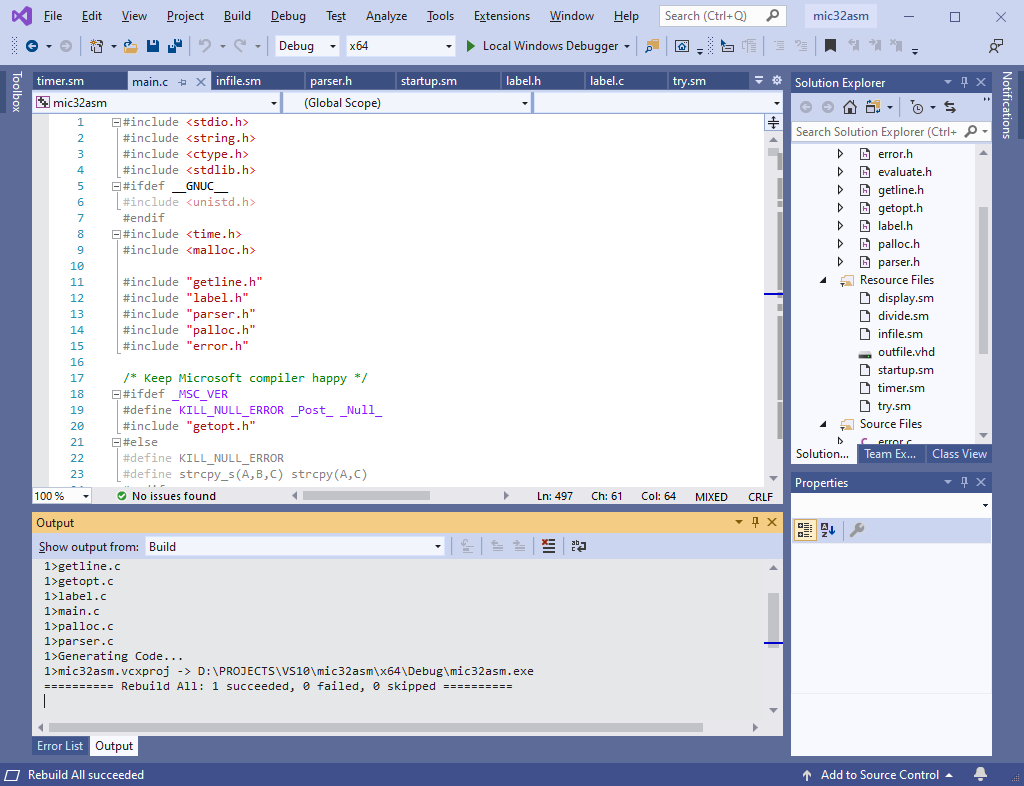
\includegraphics[width=\textwidth]{images/vs2019}
\caption{Voorbeeld van Microsoft Visual Stdio.}
\label{fig:unvs2019}
\end{figure}

We zullen in de overige paragrafen in sneltreinvaart enkelen concepten van C bespreken. In de volgende hoofdstukken wordt de taal verder uitgediept.


\section{Afdrukken op het scherm}
Laten we beginnen met een eenvoudig voorbeeld. Het programma in listing~\ref{cod:uneersteprogramma} drukt de regel \texttt{De som van 3 en 7 is 10} op het scherm af. We zullen het programma stap voor stap doorlopen.

\begin{figure}[!ht]
\begin{lstlisting}[caption=Eerste C-programma.,label=cod:uneersteprogramma]
#include <stdio.h>

int main(void) {

    int a = 3;
    int b = 7;

    int som;

    som = a+b;

	printf("De som van %d en %d is %d\n", a, b, som);

	return 0;
}
\end{lstlisting}
\end{figure}

In regel 1 wordt een zogenoemde \textsl{header-bestand}\index{header-bestand} geladen, in dit geval het bestand \texttt{stdio.h}. We leggen zo meteen uit waarom dat nodig is.

In regel 3 wordt kenbaar gemaakt dat het programma de functie \texttt{main}\indextwo{main}{functie} heeft. Een C-programma heeft de \textsl{altijd} de functie \texttt{main}. Het (gecompileerde) programma wordt hier gestart.

In regel 5 en 6 worden twee \textsl{variabelen}\index{variabele} gedeclareerd, de variabelen \texttt{a} en \texttt{b}. Een variabele kan door het programma gebruikt worden om gegevens te bewerken. Declaratie\index{declaratie} wil zeggen dat een variabele kenbaar worden gemaakt. Bij de declaratie wordt opgegeven wat het type is van de variabele. Dit gebeurt middels het \textsl{keyword}\index{keyword} \texttt{int}, dat betekent dat \texttt{a} en \texttt{b} alleen geheeltallige getallen kan opslaan (Engels: integer). Aan de variabelen worden waarden toegekend. We noemen dit \textsl{initialisatie}\index{initialisatie} van variabelen.

In regel 8 wordt de variabele \textsl{som} gedeclareerd zonder initialisatie. Dat betekent dat op dat moment de waarde (of inhoud) van de variabele \textsl{onbekend} is. Vervolgens wordt in regel 10 de som van \texttt{a} en \texttt{b} berekend middels de \textsl{optel-operator} \texttt{+} en wordt het resultaat \textsl{toegekend}\index{toekenning} aan variabele \texttt{som.} Vanaf regel 10 is de waarde van  \texttt{som} dus 10.

In regel 12 wordt de functie \texttt{printf} aangeroepen. Deze functie is al geschreven is zit in de standard library. De functie krijgt vier \textsl{argumenten}\index{argument} mee, gegevens die in de functie verwerkt worden. Het eerste argument is een \textsl{string}\index{string}. Een string is een stukje tekst, maar we spreken meestal van een rij karakters. Daarna volgen de (waarden) van de variabelen \texttt{a}, \texttt{b} en \texttt{som}.

Het eerste argument van \texttt{printf} wordt een \textsl{format string} genoemd. Dat ligt niet in C-taal vast maar wordt algemeen gebruikt. De format string bevat karakters, zogenoemde \textsl{format specifications} en een \textsl{escape sequence}. Een format specification begint met een procentteken gevolgd door een letter. De functie \texttt{printf} gebruikt deze format specifications om de gegevens af te drukken. De eerste \texttt{\%d} zorgt ervoor dat variabele \texttt{a} wordt afgedrukt als een decimaal geheel getal. Op overeenkomstige wijze worden ook \texttt{b} en \texttt{som} afgedrukt. Aan het einde van de format string is een escape sequence te zien, in dit geval \texttt{\textbackslash n}. Dit zorgt ervoor dat een volgende afdruk wordt begonnen aan het begin van de volgende regel (Engels: newline).

In regel 14 wordt met het keyword \texttt{return} aangegeven dat het programma wordt afgesloten. Dat behoeft enige uitleg. Een (gecompileerd) programma wordt gestart door het besturingssysteem. Aan het einde wordt het programma afgesloten. Het besturingssysteem ``ruimt'' het programma op en zorgt ervoor dat het gebruikte geheugen weer vrijgegeven wordt voor volgende programma's. We kunnen aan het besturingssysteem een getal teruggeven, in dit geval 0. Het is aan het besturingssysteem om hier wat mee te doen. Gebruikelijk is om 0 terug te geven als alles goed verlopen is. Een ander getal dan 0 geeft over het algemeen aan dat er iets fout gegaan is.

Dat de return-waarde een geheel getal moet zijn, kunnen we zien aan de definitie van de functie \texttt{main}. We zien in regel 3 dat \texttt{main} een geheel getal teruggeeft (keyword \texttt{int}) en geen argumenten meekrijgt (keyword \texttt{void}).

Hoe weet de C-compiler nou hoe de functie \texttt{printf} moet worden aangeroepen? Dat wordt geregeld met een \textsl{function prototype}. We hoeven dat zelf niet op te geven want dat is al gedaan en is te vinden in het header-bestand \texttt{stdio.h}. De eerste regel geeft dus aan dat dit bestand geladen moet worden. De tekens \texttt{<} en \texttt{>} geven aan dat gezocht moet worden op een bepaalde plek in het bestandssysteem. We hoeven dat verder niet te weten.

\section{Invoer van het toetsenbord}
We kunnen het eerste programma interessanter maken door aan de gebruiker te vragen om twee gehele getallen in te voeren. Het programma is te zien in listing~\ref{cod:unscanfprogramma}. We springen eerst naar regel 14 waar de functie \texttt{scanf} ervoor zorgt dat een geheel getal wordt ingelezen van het toetsenbord en in variabele \texttt{a} wordt gezet.
%
\begin{figure}[!ht]
\begin{lstlisting}[caption=Invoer van de gebruiker opvragen.,label=cod:unscanfprogramma]
#include <stdio.h>

/* Make Visual Studio happy */
#define scanf scanf_s

int main(void) {

    int a;
    int b;

    int som;

    printf("Geef een getal: ");
    scanf("%d", &a);

    printf("Geef nog een getal: ");
    scanf("%d", &b);

    som = a + b;

    printf("De som van %d en %d is %d\n", a, b, som);

    return 0;
}
\end{lstlisting}
\end{figure}
%
De format specifier \texttt{\%d} hadden we al eerder gezien, maar de constructie \texttt{\&a} is nieuw. De ampersand (\texttt{\&}) zorgt ervoor dat aan de functie \texttt{scanf} het \textsl{adres} van variabele \texttt{a} meegegeven wordt. Het adres van de variabele is de plek waar de variabele in het geheugen ligt. Op deze manier kan \texttt{scanf} de informatie op je juiste plek zetten. In regel 17 wordt hetzelfde gedaan voor variabele \texttt{b}. We drukken voor het inlezen nog even netjes af hoe de gebruiker moet handelen.

\begin{remarkbox}[Opmerking]
De Microsoft C-compiler bestempelt \texttt{scanf} als ``onveilig''. Een compilatie met \texttt{scanf} zal eindigen met een foutmelding. In plaats daarvan moet de functie \texttt{scanf\_s} worden gebruikt. Helaas ondersteunen andere compilers deze functie niet. Dat zal resulteren in een programma dat niet door iedere compiler kan worden vertaald. Om het probleem te omzeilen hebben we gebruik gemaak van een \textsl{macro}. In regel 4 definieren we dat het woord \texttt{scanf} vervangen moet worden door \texttt{scanf\_s}. Op andere compilers, bijvoorbeeld de GNU-C compiler, moet deze regel verwijderd worden. Overigens wordt op vele fora gewaarschuwd voor de onveiligheid van \texttt{scanf} en worden alternatieven gegeven. Wij gebruiken \texttt{scanf} hier wel \textsl{for the sake of simplicity}. Het is beter om \texttt{scanf} te vermijden.
\end{remarkbox}


